As mentioned in earlier sections, an annotation can either be a point annotation or an object annotation. A point annotation is an instance of a prefab 
called \texttt{SphereAnnotation} and is instantiated and added to the scene at the point where the raycast hits a collider (assuming the range threshold isn't surpassed).  
The \texttt{SphereAnnotation} prefab includes a sphere mesh, sphere collider, mesh renderer and shader, and effectively looks like a small shining orb.
An object annotation functions a little differently as no new object is added to the scene to represent the annotation. Instead, the annotation is attached to the 
object itself and the object's material ("color") is changed to show that the object has an annotation attached. Although these two annotation types differs in this respect 
they both are based on the \texttt{AnnotationInformation} class, which is a component in both the \texttt{AnnotationSphere} prefab and the annotated objects. 

In the current implementation \texttt{AnnotationInformation} is a pretty simplistic and limited class, but can easily be extended to include a lot of other functionality. 
Prehaps the most essential class member is the string variable \texttt{text}, which is simply the string value of the annotation.
This value is read when the annotation form opens (i.e the user starts editting an annotation) and displayed in the annotation form text box. 
If the user exits the annotation form by clicking the submit button the text value is replaced/updated with what's currently in the text box. 
In addition to this, the \texttt{AnnotationInformation} class also contain a material-list called \texttt{annotationMaterials} and a material reference called
\texttt{previousMaterial}. \texttt{annotationMaterials} is a list of the available materials to the annotation and is utilzed to look up which material to use for the annotation, 
e.g.~when the user changes the annotation's priority (different priorities have different colors). 
\texttt{previousMaterial} holds a reference to the previous material the annotation had, and is most commonly used in object annotations to "remember" the original material 
(since annotating an object overrides its materials), in cases where the object annotation is deleted.  

\texttt{AnnotationInformation} also contains a destroy function, called \texttt{Destroy}, which is used to delete annotations (i.e removing them from the scene).

%About how annotations are implemented

\subsection{Annotation Categories}
As mentioned earlier an annotation can have one of the following labels or categories: "Information", "Warning" or "Error", selectable in the annotation form.
These categories or labels were created to reflect the nature of an annotation in a design review settings. 
The information-category is meant for general remarks, the warning-category for potential issues and things that should be improved, and the
error-category for design aspects that needs to be changed for the design to be approved. To make this annotation distinction clear to the user
the annotation's material ("color") is changed depending on the category it belongs to. In the implementation the information-category is
the default category, i.e the category an annotation belongs to upon creation, and has the color teal. The warning-category has the color yellow and
the error-category has the color red (see~\vref{annotation_colors}).

\begin{figure}%[h!] %[H]
	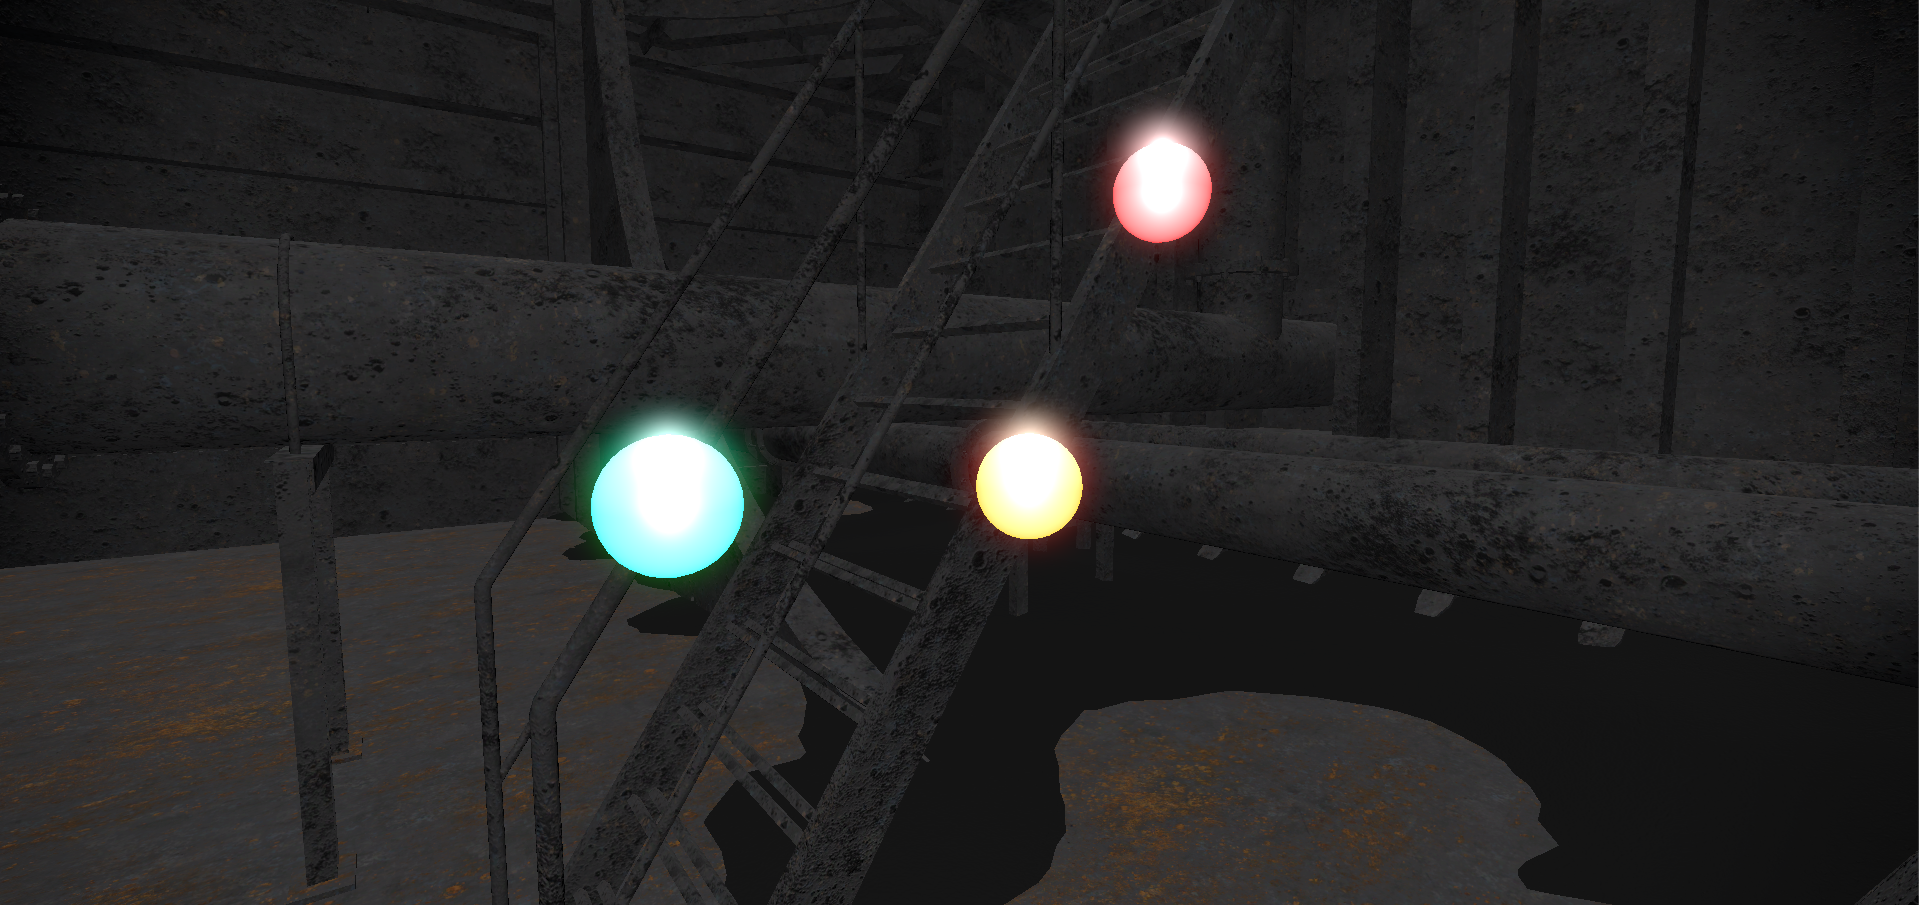
\includegraphics[width=\linewidth]{pictures/screenshots/annotations/point_annotation_colors.png}
	\caption[The Annotation Category Colors]{The Annotation Category Colors. a) Is an information-annotation and is colored in teal. 
			b) Is a warning-annotation and is colored in yellow. c) Is an error-annotation and is colored in red.}
	\label{fig:annotation_colors}
\end{figure} 

\subsection{Annotation Visibility Levels}
\label{sec:annotations}
Annotation visibiliy levels can be accessed through the menu, by clicking the "Annotation Visibility" button in the root menu, 
and decides how annotations appear in the virtual world. This includes choosing between three annotation presentation modes: "Always visible", "Visible with LOS" and 
"Invisible", with the "Always visible" setting being used by default. 
The user can from this menu also choose whether to use a glow effect on the annotation or not. 
As was mentioned in the camera rigs sections (\ref{sec:camera_rigs}), this is 
accomplished by manipulating the annotation camera in the active rig, and more specifically its culling mask and clear flags. 
This is done in the \texttt{AnnotationVisibility} script, which is partly shown in table~\vref{table:annotation_visibility_code}.

\begin{figure}%[h!] %[H]
	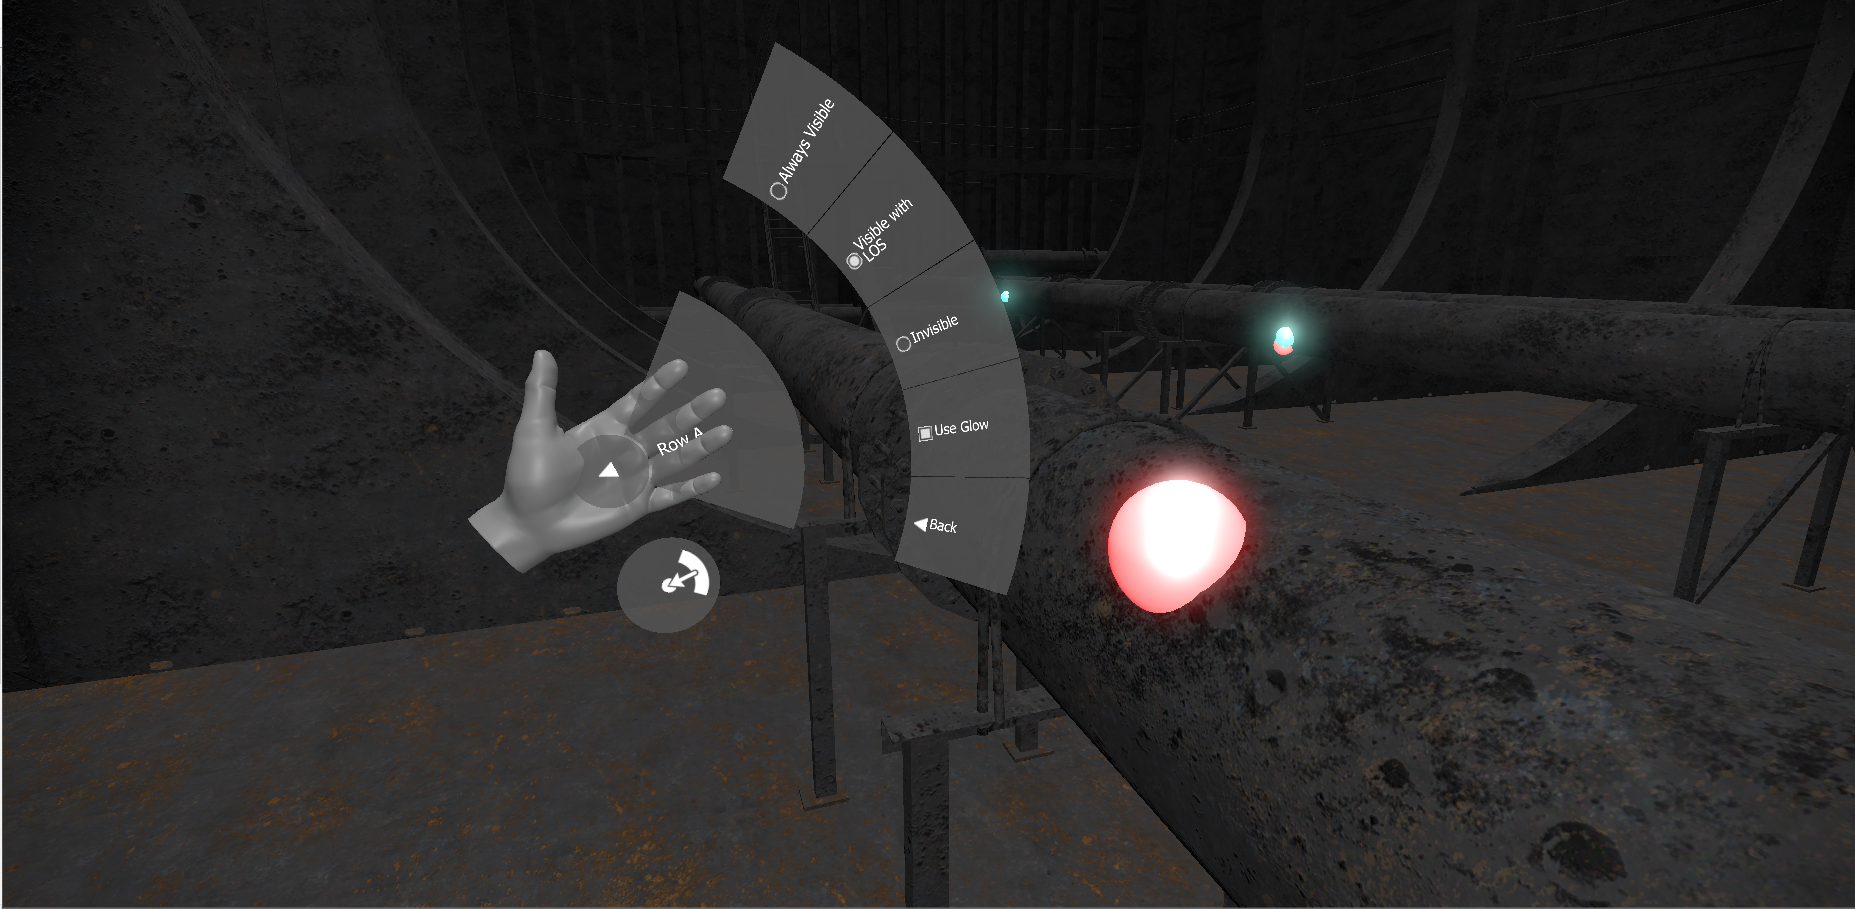
\includegraphics[width=\linewidth]{pictures/screenshots/annotation_visibility/annotation_visibility_options.png}
	\caption[The Annotation Visibility Submenu]{The user can decide three different annotation visibility settings in the Annotation Visibility Submenu.}
	\label{fig:annotation_visibility_options}
\end{figure} 

\subsubsection{Always Visible}
As mentioned in~\vref{sec:camera_rigs} the main camera's culling mask includes (and thus renders) every layer except the 
annotation layer (actually called "AnnotationSphere" in implementation), while the annotation camera, only renders
the annotation layer (\texttt{CullingMask = {SphereAnnotation}}). The output of these two cameras is combined by rendering the main camera first, and
then render the annotation camera and put its results "on top of" the main camera's output.
To ensure that the annotation camera's output doesn't overwrite the entire output of the main camera,
so only the annotation-cameras output would be shown, we have to use a different clear flag for the annotation camera than we would in a single-camera setup. 

The main camera uses a clear flag called "Solid Color", which
effectivly clears any empty portions of the screen by displaying a certain background color. 
If there is nothing for the camera to render (i.e no object in front of the camera on a layer which is included in the camera's culling mask) only this background color 
will be shown. If this clear flag were used on the annotation camera everything on the frame, except annotation models, would be this background color. 
Because of this another clear flag, called "Depth only", is used on the annotation camera. This clear flag only clears the depth buffer and not the color buffer as is done 
in with the "Solid Color"-flag. It also doesn't overwrite anything from the frames produced by other cameras 
unless it captures an object that is on a layer thats in the cameras culling mask. This effectivly means that annotations, picked up by the annotation camera, is effectly drawn
over the pixels that were produced by the main camera, effectivly removing or obstructing the parts of the model that would otherwise obstruct the annotation from the user.
This makes it so annotation are visible from all angles and distances with the "Always visible" setting active. 

\begin{figure}%[h!] %[H]
	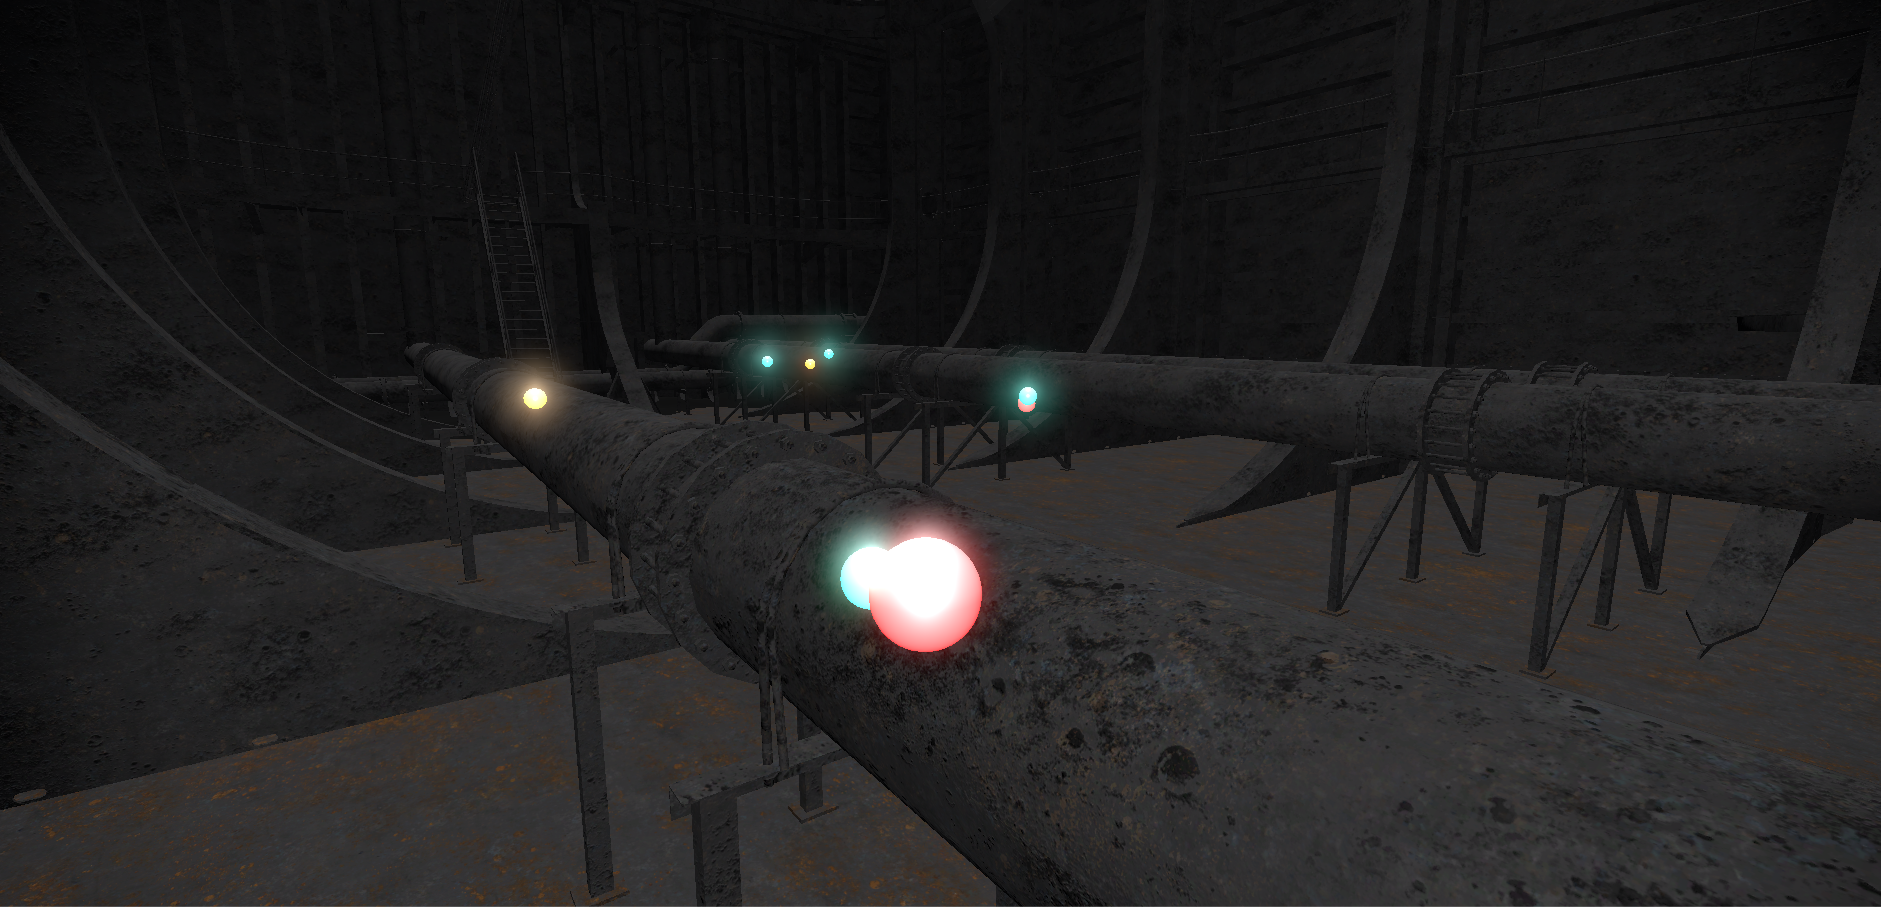
\includegraphics[width=\linewidth]{pictures/screenshots/annotation_visibility/always_visible.png}
	\caption[Annotation always visible]{When selecting the "Always visible" option in the Annotation Visibility Submenu annotations are not occluded and thus always visible, 
	even through other objects.}
	\label{fig:always_visible}
\end{figure} 

\subsubsection{Visible with Line Of Sight}
As mentioned earlier the "Always visible" option is the default in the application. This is meant to make it more easy to keep track of the different annotations 
present in the model. This seems like a good option with relatively few annotation, but can probably be distracting if the number or concentration of annotations 
grow beyond a certain size. Because of this the "Visible with LOS" (Visible with Line of Sight) option was developed to give the user the option to 
disable the "annotation are always visible"-functionality and instead only see annotation if they are directly in the line of sight.

The "Visible with LOS" option in the menu changes the behavior outlined in the previous section by some degree.
It keeps the same culling mask configurations as in the "Always visible" setting, but changes the annotation camera's clear flag to the "Nothing flag".
This flag will leave colors and depth buffer from the previous frame, which is produced by the main camera, and thus not clear anything. 
Because the depth buffer isn't cleared, as is the case with the "Solid Color" and "Depth Only" flags, objects rendered by the main camera can now
obstruct objects rendered by the annotation camera, thus giving the "normal" line of sight requirement for seeing objects. 

\subsubsection{Invisible}
To enable the user to hide annotation all together the "Annotation Visibility" submenu also offers an invisible-option. 
This option simply removed the annotion layer from the annotation camera's culling mask, thus leaving the annotation camera to render nothing.
The clear flag is kept in its current state as neither the "Depth only" or "Nothing" flag interferes with the frames produced from the main camera
when nothing is produced by the annotation camera.

\begin{figure}%[h!] %[H]
	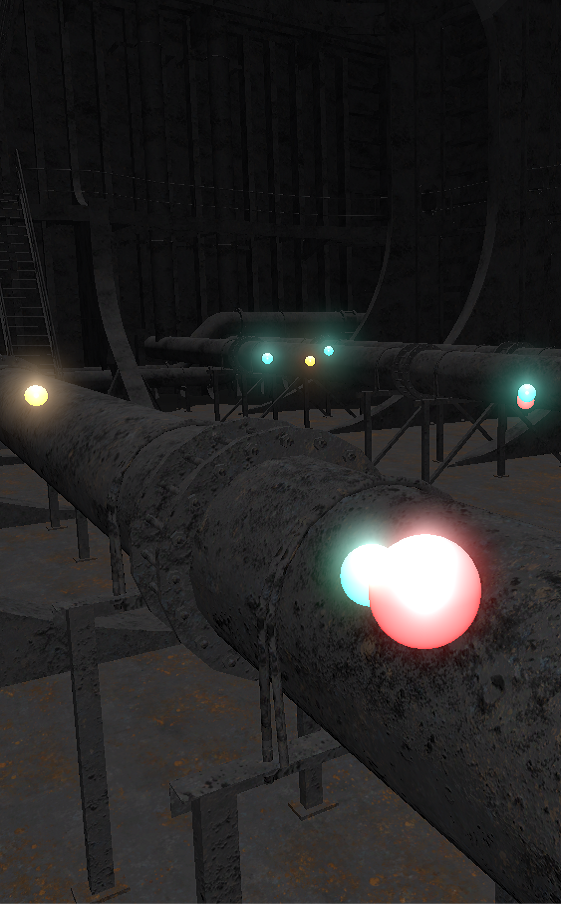
\includegraphics[width=0.32\linewidth]{pictures/screenshots/annotation_visibility/side_by_side/always_visible_small.png}
	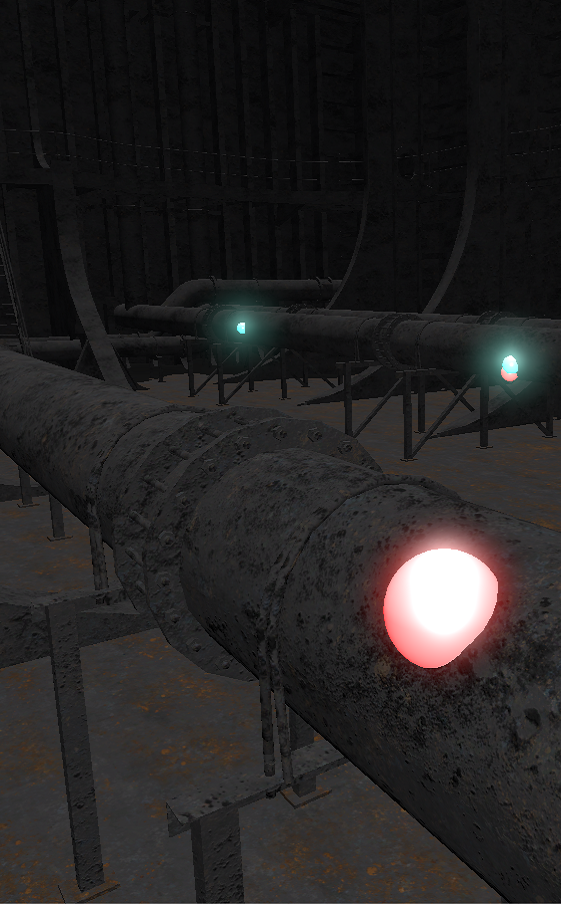
\includegraphics[width=0.32\linewidth]{pictures/screenshots/annotation_visibility/side_by_side/LOS_visible_small.png}
	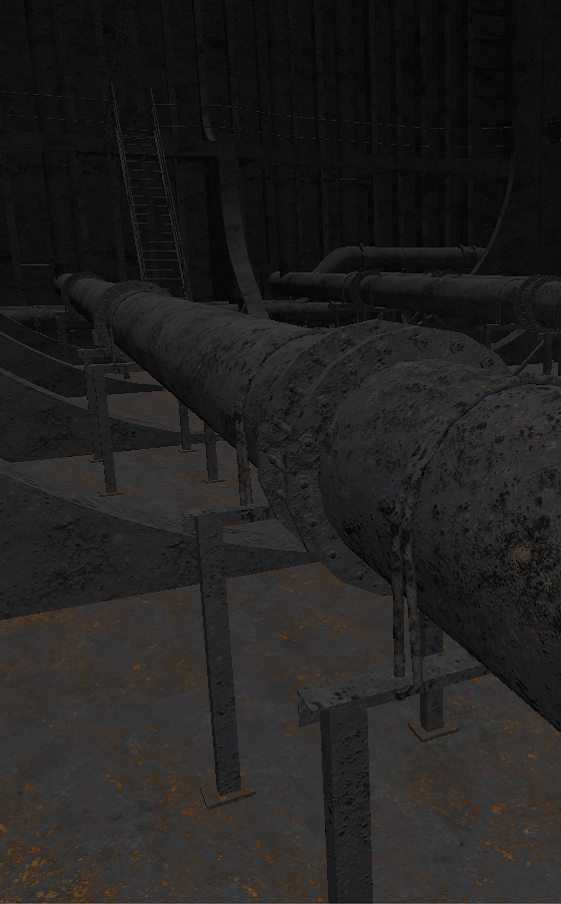
\includegraphics[width=0.32\linewidth]{pictures/screenshots/annotation_visibility/side_by_side/invisible_small.png}
	\caption[Annotation visibility levels comparison]{A side-by-side comparison of the annotation visibility levels. These three pictures are taken with the same camera position
	and orientation using different visibility settings. 	
	"Always visible" option (left): Annotations are not occluded and thus always visible, even through other objects. % like the pipes present in this picture. 	
	"Visible with LOS" option (middle): Annotations are only visible with line of sight. 	
	"Invisible" option (right): Annotations are not visible.}
	\label{fig:visibility_comparison}
\end{figure} 